\documentclass[11pt]{article}\usepackage[]{graphicx}\usepackage[]{color}
%% maxwidth is the original width if it is less than linewidth
%% otherwise use linewidth (to make sure the graphics do not exceed the margin)
\makeatletter
\def\maxwidth{ %
  \ifdim\Gin@nat@width>\linewidth
    \linewidth
  \else
    \Gin@nat@width
  \fi
}
\makeatother

\definecolor{fgcolor}{rgb}{0.345, 0.345, 0.345}
\newcommand{\hlnum}[1]{\textcolor[rgb]{0.686,0.059,0.569}{#1}}%
\newcommand{\hlstr}[1]{\textcolor[rgb]{0.192,0.494,0.8}{#1}}%
\newcommand{\hlcom}[1]{\textcolor[rgb]{0.678,0.584,0.686}{\textit{#1}}}%
\newcommand{\hlopt}[1]{\textcolor[rgb]{0,0,0}{#1}}%
\newcommand{\hlstd}[1]{\textcolor[rgb]{0.345,0.345,0.345}{#1}}%
\newcommand{\hlkwa}[1]{\textcolor[rgb]{0.161,0.373,0.58}{\textbf{#1}}}%
\newcommand{\hlkwb}[1]{\textcolor[rgb]{0.69,0.353,0.396}{#1}}%
\newcommand{\hlkwc}[1]{\textcolor[rgb]{0.333,0.667,0.333}{#1}}%
\newcommand{\hlkwd}[1]{\textcolor[rgb]{0.737,0.353,0.396}{\textbf{#1}}}%
\let\hlipl\hlkwb

\usepackage{framed}
\makeatletter
\newenvironment{kframe}{%
 \def\at@end@of@kframe{}%
 \ifinner\ifhmode%
  \def\at@end@of@kframe{\end{minipage}}%
  \begin{minipage}{\columnwidth}%
 \fi\fi%
 \def\FrameCommand##1{\hskip\@totalleftmargin \hskip-\fboxsep
 \colorbox{shadecolor}{##1}\hskip-\fboxsep
     % There is no \\@totalrightmargin, so:
     \hskip-\linewidth \hskip-\@totalleftmargin \hskip\columnwidth}%
 \MakeFramed {\advance\hsize-\width
   \@totalleftmargin\z@ \linewidth\hsize
   \@setminipage}}%
 {\par\unskip\endMakeFramed%
 \at@end@of@kframe}
\makeatother

\definecolor{shadecolor}{rgb}{.97, .97, .97}
\definecolor{messagecolor}{rgb}{0, 0, 0}
\definecolor{warningcolor}{rgb}{1, 0, 1}
\definecolor{errorcolor}{rgb}{1, 0, 0}
\newenvironment{knitrout}{}{} % an empty environment to be redefined in TeX

\usepackage{alltt}
\usepackage{amsmath}
\usepackage{amssymb}
\usepackage[intoc,english]{nomencl}
\usepackage{graphicx}
\usepackage{bm}
\usepackage{float}
\usepackage[margin=1in]{geometry}
\usepackage[section]{placeins}
\usepackage{biblatex}
\usepackage{comment}
\usepackage{xcolor}
\usepackage[toc,page]{appendix}
\usepackage[acronym]{glossaries}
\renewcommand{\nomname}{List of Abbreviations and Symbols Used}
\makenomenclature
\makeglossaries
\renewbibmacro{in:}{}
\addbibresource{spam.bib}

\newacronym{tmb}{TMB}{Template Model Builder}
\newacronym{ad}{AD}{Automatic Differentation}
\newacronym{mle}{MLE}{Maximum Likelihood Estimation}
\newacronym{la}{LA}{Laplace Approximation}
\newacronym{cdf}{CDF}{Cumulative Distribution Function}
\newacronym{pdf}{PDF}{Probability Density Function}
\newacronym{spam}{SPAM}{St. Pierre bank Assessment Model}
\newacronym{fda}{FDA}{Functional Data Analysis}
\newacronym{fpca}{FPCA}{Functional Principal Component Analysis}
\newacronym{pca}{PCA}{Principal Component Analysis}
\newacronym{fpc}{FPC}{Functional Principal Components}
\newacronym{ssb}{SSB}{Spawning Stock Biomass}
\newacronym{dfo}{DFO}{Fisheries and Oceans Canada}
\newacronym{gcv}{GCV}{Generalized Cross Validation}

\specialcomment{DrF}{\begingroup\ttfamily\color{blue}}{\endgroup}

\specialcomment{Me}{\begingroup\ttfamily\color{red}}{\endgroup}
%Control for the comments package
%\excludecomment{DrF}
\IfFileExists{upquote.sty}{\usepackage{upquote}}{}
\begin{document}





\title{St. Pierre bank assessment model}
\author{Jonathan Babyn}
\date{\today}
\maketitle

\tableofcontents
\newpage

\printnomenclature

\section{Introduction}

\section{Model Design}

\acrshort{spam} uses the standard population dynamics model for the abundance at age $a$ in year $y$ as,
\begin{equation}\label{abun}
  N_{a,y} = N_{a-1,y-1}\exp(-Z_{a-1,y-1})
\end{equation}
and extends it for the plus group $A$, comprising all fish at and above age $A$ with
\begin{equation}\label{abunPlus}
	N_{a,y} = N_{a-1,y-1}\exp(-Z_{a-1,y-1}) + N_{A,y-1}\exp(-Z_{A,y-1}).	
\end{equation}
Total morality $Z_{a,y}$ was assumed to be of the form
\begin{equation}
Z_{a,y} = F_{a,y} + M_{a,y},	
\end{equation}
with $F_{a,y}$ being fishing mortality and $M_{a,y}$ natural mortality which was fixed to be a constant 0.2.
\section{Smoothing Maturities and Weights}

Two important pieces for calculating \acrshort{ssb} are the weights used and maturity ogives. The maturity ogives provided are the output of a logistic regression run and updated each year from fish that have had their otoliths aged, lengths measured and maturity status determined. This results in very noisy maturity data set for each age group. For both the commercial and stock weights, output from a cohort model going from 1983 to 2016 were provided, along with commercial and stock weights from 1959 to 2014 and 1959 to 2017 respectively provided by \acrshort{dfo}. The weights provided by \acrshort{dfo} are noisy, and values prior to 1977 are identical and likely copy and pasted from some mean weights derived at some point. Neither of these situations are ideal. The weights either need to be extended thirty back into the past or improved. While the \acrshort{dfo} provided weights unfortunately do not have real observations prior to 1977, the values provided at least seem consistent when compared with the output of the cohort model weights. I chose to try and deal with the noise in the \acrshort{dfo} provided weights rather than extend the other weights back as the \acrshort{dfo} weights are based on actual commercial sampling efforts rather than being based off research vessel survey data and weight length relationships.

 Both the maturities and weights were smoothed using \acrfull{fpca}. \acrshort{fpca} is a non-parametric technique that has been used to perform noise reduction on curve like data\cite{ramsay2007applied}. \acrshort{fpca} has at least been at least applied to fisheries data in the context of evaluating spatio-temporal patterns in the data\cite{embling_2012} but it has not to the author's knowledge been applied to fisheries weight or growth data. The noise reduction is done by breaking the data down into it's mean function $\mu(t)$, eigenfunctions $\phi_k(t)$ and \acrfull{fpc}, $\xi_{ki}$ and keeping only the number of \acrshort{fpc}s that explain most of the variation in the data.  Further details on \acrshort{fpca} and this process can be seen in Appendix \ref{afpca}.



For the maturities, the logit was taken and the \acrshort{fpca} performed in logit space to ensure that maturity proportions would continue to lie between 0 and 1 after smoothing. The FPCA was performed with each age group being considered an observation measured at each year. Smoothing was allowed on the mean function and a user selected bandwidth of 14 was chosen which removed many of the peaks and valleys. The diagnostic plots of the \acrshort{fpca} performed on the maturities showcasing the mean function, first three eigenfunctions, fraction of variance explained by each \acrshort{fpc} are seen in Figure \ref{fig:matFPCAd}. Over 90\% of the variance is explained by the first \acrshort{fpc}, because of this only the first \acrshort{fpc} was used in creating the smoothed data. Plots comparing the smoothed and raw versions of the maturities by age and year are in Figure \ref{matFPCAp}.

For the weights the years were treated as observations and the age groups as measurement points. Here the mean function was automatically smoothed using \acrfull{gcv}. The diagnostic plots for the FPCA on the commercial weights are in Figure \ref{fig:weightFPCAd}, the diagnostic plots for the stock weights look very similar and are not included here. On the weights data, again over 90\% of the variation is explained by a single \acrshort{fpc}. Looking at the data represented with a single \acrshort{fpc} revealed a distinct gap between the bulk of the data. This gap almost perfectly separates the weights into pre-1994 and post-1994 groups, with a further more obvious recent downshift in weights that occurred after 2011. This grouping along with plots of the raw and smoothed weights are shown in Figure \ref{fig:weightFPCAp}. A k-means with $k=3$ clustering algorithm was also applied to the \acrshort{fpc}s of the weights to try and find groupings that way. With the repeated data from 1977 prior removed, almost the same groups as seen in Figure \ref{fig:weightFPCAp} were found on the commercial data and groups that mostly split the stock weight data into pre-1994 and post-1994 clusters..

 The \acrshort{dfo} provided weights were only provided for ages three through fourteen and needed to be extended for ages 1,2, 15 and 16. This was done by extrapolating the mean function and eigenfunctions of the \acrshort{fpca} using splines at those points. While extrapolating beyond the boundaries is not ideal, the mean function and the first eigenfunction seem well behaved at the boundaries and the imputed values seem reasonable. 




\begin{knitrout}
\definecolor{shadecolor}{rgb}{0.969, 0.969, 0.969}\color{fgcolor}\begin{figure}
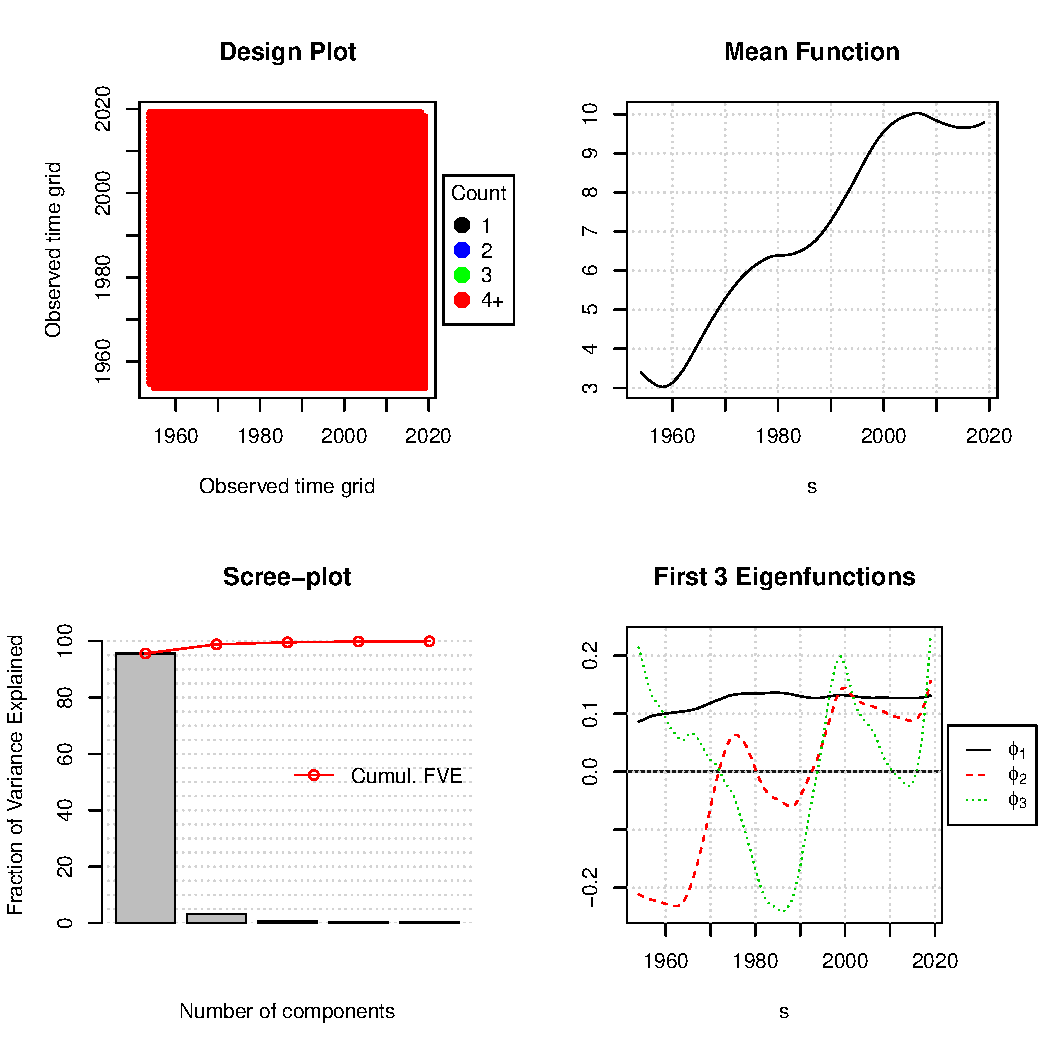
\includegraphics[width=\maxwidth]{figure/matFPCAd-1} \caption[Diagnostic plots the FPCA performed on maturity proportions]{Diagnostic plots the FPCA performed on maturity proportions. Top right shows the smoothed mean function, bottom right shows the first 3 eigenfunctions, bottom left the fraction of variance explained by each FPC, top left is the number of measurements at each grid point}\label{fig:matFPCAd}
\end{figure}


\end{knitrout}

\begin{knitrout}
\definecolor{shadecolor}{rgb}{0.969, 0.969, 0.969}\color{fgcolor}\begin{figure}
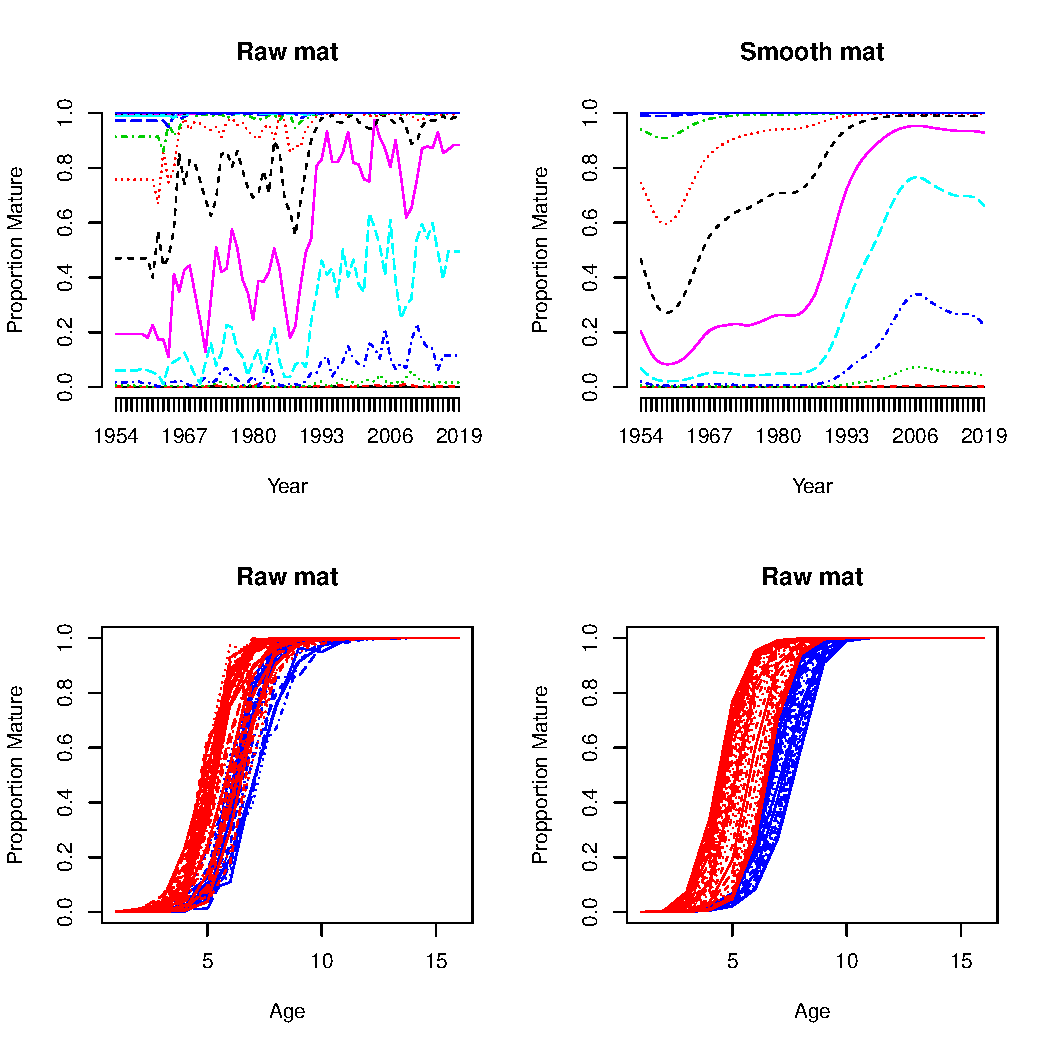
\includegraphics[width=\maxwidth]{figure/matFPCAp-1} \caption[Raw and smoothed maturity proportion curves both by age and by year]{Raw and smoothed maturity proportion curves both by age and by year. For the proportions by age, red curves are those post-1980, blue are pre-1980 suggesting later cohorts mature faster.}\label{fig:matFPCAp}
\end{figure}


\end{knitrout}


\begin{knitrout}
\definecolor{shadecolor}{rgb}{0.969, 0.969, 0.969}\color{fgcolor}\begin{figure}
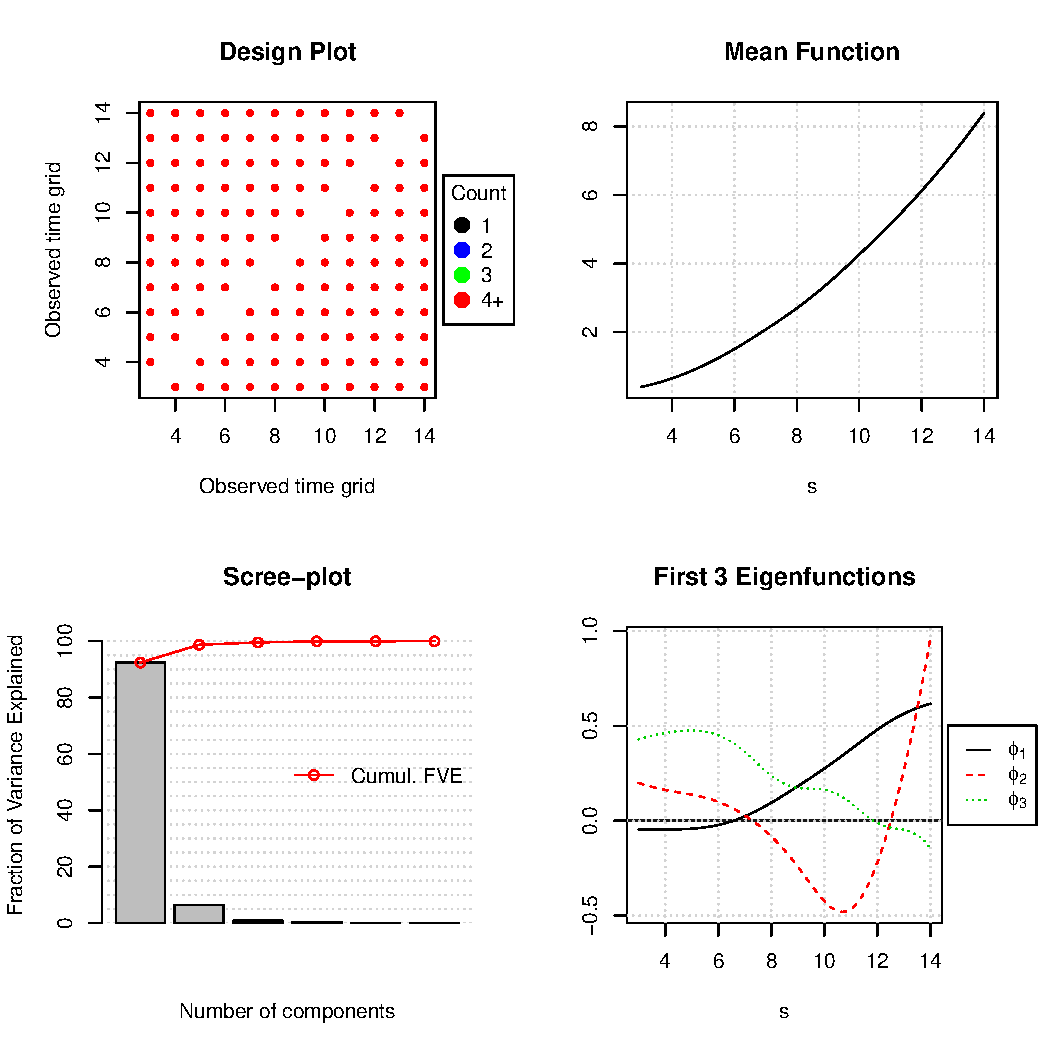
\includegraphics[width=\maxwidth]{figure/weightFPCAd-1} \caption[Diagnostic plots of the FPCA performed on the commercial weights]{Diagnostic plots of the FPCA performed on the commercial weights.}\label{fig:weightFPCAd}
\end{figure}


\end{knitrout}

\begin{knitrout}
\definecolor{shadecolor}{rgb}{0.969, 0.969, 0.969}\color{fgcolor}\begin{figure}
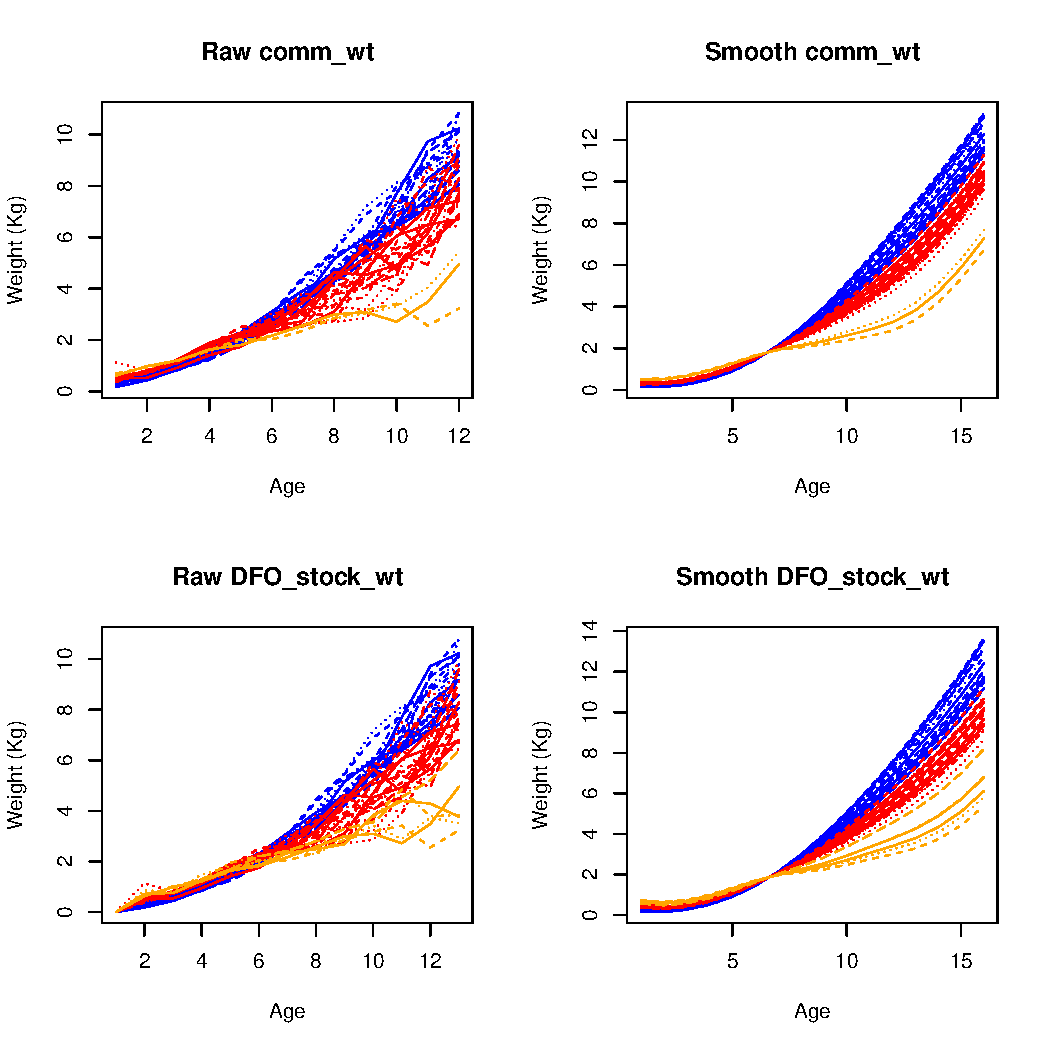
\includegraphics[width=\maxwidth]{figure/weightFPCAp-1} \caption[Raw DFO provided commercial weights vs]{Raw DFO provided commercial weights vs. those smoothed by FPCA. Blue curves are those pre-1994, Red are post-1994 and orange are post-2011. Ages 2,3,15 and 16 weights were created by extrapolating the mean function and eigenfunctions to those points using splines and then imputing based on those extrapolations.}\label{fig:weightFPCAp}
\end{figure}


\end{knitrout}

\begin{appendices}
\section{Numerically stable logged normal cumulative distribution function derivatives in TMB}\label{astable1}
\texttt{\acrshort{tmb}} uses \acrfull{ad} to generate the first and second derivatives which are used to help with both performing \acrshort{mle} for parameters and integrating random effects out of the likelihood with the \acrfull{la}. \texttt{\acrshort{tmb}} accomplishes this with a mixture of forward and reverse \acrshort{ad} accumulation modes. Further details on \acrshort{ad} can be seen in Fournier et al\cite{Fournier_2012}. \texttt{\acrshort{tmb}} automatically tries to determine the derivatives of the user's template. However, it can not automatically determine the most numerically stable form of the derivative which can often be necessary when working with extremely small values that can commonly occur when working with probabilities. \texttt{\acrshort{tmb}} also includes the ability to manually define the forward and reverse modes for a given function to overcome this limitation using atomic functions. By default \texttt{\acrshort{tmb}} includes a built in atomic version of the normal \acrshort{cdf}, \texttt{pnorm} based on the version in \texttt{R}'s \texttt{C} language math library. This built-in version does not support the ability to return a logged value of the probability and shares the same limitation of returning 0 or 1 for negative or positive values of standard normal $Z$ scores when $|Z| > \sim 38$ due to floating point limitations. This clearly means that for any $Z < -38$, \texttt{\acrshort{tmb}} will return a \texttt{NaN} in the gradient when trying to perform \texttt{log(pnorm(Z))} due to $\log(0)$ being negative infinity. In practice however this is actually much worse since the derivative of \texttt{log(pnorm(Z))} is 
\begin{equation}\label{derlNCDF}
	{{e^ {- {{z^2}\over{2}} }}\over{\sqrt{2\pi}\,\left({{
 \mathrm{erf}\left({{z}\over{\sqrt{2}}}\right)}\over{2}}+{{1}\over{2
 }}\right)}}
\end{equation}
and easily results in the division of two extremely small numbers. With floating point limitations this quickly becomes undefined if not handled correctly. 

I created an atomic function to specifically deal with the problem of numerical stability when trying to do \texttt{log(pnorm(Z))} and similar calculations in the objective function of \acrshort{spam} such as those done when using a censored likelihood for the detection limit for fitting the observation equations for the survey indices. This requires specifying more numerically stable versions for both the forward and reverse \acrshort{ad} modes. For the forward mode this is just the \texttt{double C++} function giving the log of the normal \acrshort{cdf} and all that requires is calling the version of \texttt{pnorm} in \texttt{R}'s \texttt{C} math library with the \texttt{give.log} flag turned on. For the reverse mode just using Equation \ref{derlNCDF} is not numerically stable due to the division. It can easily be seen that Equation \ref{derlNCDF} is equivalent to 
\begin{equation}\label{logder}
	\exp \left (\log \left({{e^ {- {{z^2}\over{2}} }}\over{\sqrt{2\pi}}}
 \right) - \log \left({{\mathrm{erf}\left({{z}\over{\sqrt{2}}}\right)}\over{2
 }}+{{1}\over{2}}\right) \right).
\end{equation}
 Working in log space is much less likely to result in under or overflow of floating point values when performing division of small numbers. Using numerically stable versions of the logged normal \acrshort{pdf} \& \acrshort{cdf}s and the form in Equation \ref{logder} results in a numerically stable reverse mode derivative for \texttt{log(pnorm(Z))}. The atomic function was wrapped in the function \texttt{pnorm4} and made available for others to use in the \texttt{C++} header file \texttt{pnorm4.hpp}. Using \texttt{pnorm4(Z)} in place of \texttt{log(pnorm(Z))} allows for running one-sided censor likelihood bounds without the need for using two runs of optimization.
 
 It's accuracy was checked by comparing the results of the gradient and hessian generated by \texttt{\acrshort{tmb}} for \texttt{pnorm4} against the numerical first and second derivatives of \texttt{pnorm4} done by the \texttt{R} software package \texttt{numDeriv} along with the brute force first and second derivatives of the normal log(\acrshort{cdf}) calculated by the open-source computer algebra system \texttt{Maxima} with 5000 digits of floating point precision. 

\subsection{Extending stability to censored bounds} 	\label{astable2}
Censored likelihood bounds pose a similar problem to the above. When using the built-in functions to add normally distributed censored log-likelihood bounds this can be done like \texttt{log(pnorm(ZU))-log(pnorm(ZU))} where \texttt{ZU} \& \texttt{ZL} are Z scores of the upper and lower bounds respectively. Just replacing the calls to \texttt{pnorm} with the more stable \texttt{pnorm4} and using the brute force approach or \texttt{logspace\_sub} to perform the subtraction is not stable either. This is because for $Z > 38$ \texttt{pnorm} will return 1, or 0 for the logged version which will then result in trying to take the log of 0, again leading to \texttt{NaN} in the gradient.

The normal CDF of the upper and lower bounds can be thought of as $\Phi(ZU)=1-\epsilon_u$ and $\Phi(ZL)=1-\epsilon_l$ where the $0 < \epsilon < 1$ and the censored log-likelihood bound is 
\begin{equation}
	\log(\Phi(ZU)-\Phi(ZL)) = \log(1-\epsilon_u-(1-\epsilon_l)) = \log(\epsilon_l-\epsilon_u). 
\end{equation}
It can also be seen that 
\begin{equation}\label{negFormm}
	\log(\Phi(-ZL)-\Phi(-ZU)) = \log(\epsilon_l-\epsilon_u) \quad \text{since} \quad \Phi(-Z) = 1-\Phi(Z) = 1-(1-\epsilon) = \epsilon.
\end{equation}
Since the problem of \texttt{NaN}s in the gradient is occurs because the relatively large value of 1 overwhelms the incredibly small values of $\epsilon$ for large positive values of Z again due to floating point limitations. This was solved by using equation \ref{negFormm} for positive values of Z instead but with probabilities returned in logged form and the subtraction done with \texttt{logspace\_sub}. This prevents the small $\epsilon$s from disappearing in the subtraction.   

Then a stable reverse mode similar to the one for \texttt{pnorm4} was made, and this was wrapped in the function \texttt{censored\_bounds}, checked for accuracy the same way and again made available for everyone to use in \texttt{pnorm4.hpp}. 

\section{Functional Principal Component Analysis}\label{afpca}

\acrfull{fda} is a branch of statistics that deals with data that takes values in an infinite dimensional or functional space. Growth and maturity curves are one-dimensional examples of functional data. Several classical statistical techniques have been extended to work with functional data, \acrfull{pca} being among them. In \acrfull{pca} the goal is to perform dimension reduction while maximizing the variation explained by each dimension, \acrfull{fpca} extends this to functional data. Let X be a random function defined on the function grid $[0,T]$ with unknown smooth mean function
\begin{equation}
E[X(t)] = \mu(t) \quad t \in [0,T],	
\end{equation}
and covariance function
\begin{equation}
\text{Cov}(X(s),X(t)) = G(s,t) \quad s,t \in [0,T].	
\end{equation}
$G(s,t)$ can be written in it's orthogonal expansion as
\begin{equation}
	G(s,t) = \sum_{k=1}^{\infty} \lambda_k \phi_k(s)\phi_k(t)
\end{equation}
 where $\lambda_k$ are the eigenvalues, and $\phi_k$ are eigenfunctions that form an othonormal basis with a unit norm. Using the orthogonal expansion allows re-writing each functional observation $X_i(t)$ in the Karhunen-Lo\`eve representation
 \begin{equation}
 X_i(t) = \mu(t) + \sum_{k=1}^{\infty} \xi_{ik}\phi_k(t) \quad \text{where} \quad \xi_{ik}= \int(X_i(t)-\mu(t))\phi_k(t)dt.
 \end{equation}
 The $\xi_{ik}$ are the \acrfull{fpc}\cite{Chiou_2014}. Like \acrshort{pca} Principal Components, \acrshort{fpc}s can also be clustered using clustering algorithms to find groups in the data. 
 
 The Karhunen-Lo\`eve representation enables a few different things. When using estimated forms of the mean function, \acrshort{fpc}s, and eigenfunctions which can be found a number of ways such as numerical integration, using a limited number of \acrshort{fpc}s that explain most of the variation in the data can be used to generate noise reduced versions of the data while keeping the parts of the process that explain the most variability\cite{ramsay2007applied}. If $L$ is the number of \acrshort{fpc} that explain for example 90\% of the variation in the data, then noise reduced observations can be made by
 \begin{equation}
 	\hat{X}_i(t) = \hat{\mu}(t) + \sum_{k=1}^{L} \hat{\xi}_{ik}\hat{\phi}_k(t).
 \end{equation}
 This same method can be used to impute missing parts of the function as well\cite{Chiou_2014}.


\end{appendices}


\printbibliography

\end{document}
